\documentclass[journal,12pt,twocolumn]{IEEEtran}
%
\usepackage{setspace}
\usepackage{textcomp}
\usepackage{gensymb}
%\doublespacing
\singlespacing

\usepackage[cmex10]{amsmath}
\usepackage{amsthm}
%\usepackage{iithtlc}
\usepackage{mathrsfs}
\usepackage{txfonts}
\usepackage{stfloats}
\usepackage{bm}
\usepackage{cite}
\usepackage{cases}
\usepackage{subfig}
%\usepackage{xtab}
\usepackage{longtable}
\usepackage{multirow}
%\usepackage{algorithm}
%\usepackage{algpseudocode}
\usepackage{enumitem}
\usepackage{mathtools}
\usepackage{steinmetz}
\usepackage{tikz}
\usepackage{circuitikz}
\usepackage{verbatim}
\usepackage{tfrupee}
\usepackage[breaklinks=true]{hyperref}
%\usepackage{stmaryrd}
\usepackage{tkz-euclide} % loads  TikZ and tkz-base
%\usetkzobj{all}
\usetikzlibrary{calc,math}
\usepackage{listings}
    \usepackage{color}                                            %%
    \usepackage{array}                                            %%
    \usepackage{longtable}                                        %%
    \usepackage{calc}                                             %%
    \usepackage{multirow}                                         %%
    \usepackage{hhline}                                           %%
    \usepackage{ifthen}                                           %%
  %optionally (for landscape tables embedded in another document): %%
    \usepackage{lscape}     
\usepackage{multicol}
\usepackage{chngcntr}
%\usepackage{enumerate}

%\usepackage{wasysym}
%\newcounter{MYtempeqncnt}
\DeclareMathOperator*{\Res}{Res}
%\renewcommand{\baselinestretch}{2}
\renewcommand\thesection{\arabic{section}}
\renewcommand\thesubsection{\thesection.\arabic{subsection}}
\renewcommand\thesubsubsection{\thesubsection.\arabic{subsubsection}}

\renewcommand\thesectiondis{\arabic{section}}
\renewcommand\thesubsectiondis{\thesectiondis.\arabic{subsection}}
\renewcommand\thesubsubsectiondis{\thesubsectiondis.\arabic{subsubsection}}

% correct bad hyphenation here
\hyphenation{op-tical net-works semi-conduc-tor}
\def\inputGnumericTable{}                                 %%

\lstset{
%language=C,
frame=single, 
breaklines=true,
columns=fullflexible
}
\newenvironment{amatrix}[1]{%
  \left(\begin{array}{@{}*{#1}{c}|c@{}}
}{%
  \end{array}\right)
}
\DeclarePairedDelimiter\abs{\lvert}{\rvert}%
\DeclarePairedDelimiter\norm{\lVert}{\rVert}%

% Swap the definition of \abs* and \norm*, so that \abs
% and \norm resizes the size of the brackets, and the 
% starred version does not.
\makeatletter
\let\oldabs\abs
\def\abs{\@ifstar{\oldabs}{\oldabs*}}
%
\let\oldnorm\norm
\def\norm{\@ifstar{\oldnorm}{\oldnorm*}}
\makeatother

\newtheorem{theorem}{Theorem}[section]
\newtheorem{problem}{Problem}
\newtheorem{proposition}{Proposition}[section]
\newtheorem{lemma}{Lemma}[section]
\newtheorem{corollary}[theorem]{Corollary}
\newtheorem{example}{Example}[section]
\newtheorem{definition}[problem]{Definition}
%\newtheorem{thm}{Theorem}[section] 
%\newtheorem{defn}[thm]{Definition}
%\newtheorem{algorithm}{Algorithm}[section]
%\newtheorem{cor}{Corollary}
\newcommand{\BEQA}{\begin{eqnarray}}
\newcommand{\EEQA}{\end{eqnarray}}
\newcommand{\define}{\stackrel{\triangle}{=}}
\bibliographystyle{IEEEtran}
%\bibliographystyle{ieeetr}
\providecommand{\mbf}{\mathbf}
\providecommand{\pr}[1]{\ensuremath{\Pr\left(#1\right)}}
\providecommand{\qfunc}[1]{\ensuremath{Q\left(#1\right)}}
\providecommand{\sbrak}[1]{\ensuremath{{}\left[#1\right]}}
\providecommand{\lsbrak}[1]{\ensuremath{{}\left[#1\right.}}
\providecommand{\rsbrak}[1]{\ensuremath{{}\left.#1\right]}}
\providecommand{\brak}[1]{\ensuremath{\left(#1\right)}}
\providecommand{\lbrak}[1]{\ensuremath{\left(#1\right.}}
\providecommand{\rbrak}[1]{\ensuremath{\left.#1\right)}}
\providecommand{\cbrak}[1]{\ensuremath{\left\{#1\right\}}}
\providecommand{\lcbrak}[1]{\ensuremath{\left\{#1\right.}}
\providecommand{\rcbrak}[1]{\ensuremath{\left.#1\right\}}}
\providecommand{\system}{\overset{\mathcal{H}}{ \longleftrightarrow}}
	%\newcommand{\solution}[2]{\textbf{Solution:}{#1}}
\newcommand{\solution}{\noindent \textbf{Solution: }}
\newcommand{\cosec}{\,\text{cosec}\,}
\providecommand{\dec}[2]{\ensuremath{\overset{#1}{\underset{#2}{\gtrless}}}}
\newcommand{\myvec}[1]{\ensuremath{\begin{pmatrix}#1\end{pmatrix}}}
\newcommand{\mydet}[1]{\ensuremath{\begin{vmatrix}#1\end{vmatrix}}}
%\numberwithin{equation}{section}
\numberwithin{equation}{subsection}
%\numberwithin{problem}{section}
%\numberwithin{definition}{section}
\makeatletter
\@addtoreset{figure}{problem}
\makeatother
\let\StandardTheFigure\thefigure
\let\vec\mathbf
\usepackage{mathtools, nccmath}
\begin{document}
\begin{center}
\huge Assignment 5\\
\large Lt Cdr Atul Mahajan\\
\large AI20MTECH13001\\
\end{center}
\begin{abstract}
This document is about tracing a Curve
\end{abstract}
Download all Latex code from 
\begin{lstlisting}
https://github.com/Atul191/Assignment 5
\end{lstlisting}
\section{problem}
Trace the following 
\begin{align}
    x^2-3xy+y^2+10x-10y+21=0 \label{eq 1}
\end{align}
\section{Solution}
The given quadratic equation can be written in the matrix form as
\begin{align}
    \vec{x}^T\myvec{1&-\frac{3}{2}\\-\frac{3}{2}&1}\vec{x}+2\myvec{5&-5}\vec{x}+21=0\label{eq:1}
\end{align}
Calculating the parameters,we get
\begin{align}
    \mydet{\vec{V}}=\mydet{1&-\frac{3}{2}\\-\frac{3}{2}&1}=-\frac{5}{4}
\end{align}
Since, $\mydet{\vec{V}} < 0$, therefore the given  equation represents a hyperbola.\par
The characteristic equation of $\vec{V}$ will be
\begin{align}
    \mydet{\vec{V}-\lambda\vec{I}}&=\mydet{1-\lambda&-\frac{3}{2}\\-\frac{3}{2}&1-\lambda}=0\\
    &\implies 4\lambda^2-8\lambda-5 =0 \\
   &\implies\lambda_1=\frac{5}{2},\lambda_2=-\frac{1}{2}\label{eq 2}
\end{align}
The eigen vector $\vec{p}$ is given by
\begin{align}
 \vec{V}\vec{p}=\lambda\vec{p}
\end{align}
\begin{align}
  \implies{\vec{V}-\lambda\vec{I}} \vec{p}=0 \label{eq 3} 
\end{align}
For $\lambda_1 = \frac{5}{2} $
\begin{align}
\vec{V}-\lambda\vec{I}= \myvec{1-\frac{5}{2}&-\frac{3}{2}\\-\frac{3}{2}&1-\frac{5}{2}}
    \end{align}
    \begin{align}
 =\myvec{-\frac{3}{2}&-\frac{3}{2}\\-\frac{3}{2}&-\frac{3}{2}}
    \end{align}
    \begin{align}
    \myvec{-\frac{3}{2}&-\frac{3}{2}\\-\frac{3}{2}&-\frac{3}{2}}\xleftrightarrow{R_2=R_2-R_1}\myvec{-\frac{3}{2}&-\frac{3}{2}\\ 0 &0}
\end{align}
 \begin{align}
    \xleftrightarrow{R_1=R_1/-\frac{3}{2}}\myvec{1&1\\ 0 &0}\label {eq 4}
   \end{align}
Substituting \eqref{eq 4} in \eqref{eq 3} we get 
\begin{align}
   \vec{p_1}=\myvec{-1\\1}
\end{align}
Therefore the normalized eigen vector will be
\begin{align}
    \vec{p_1}=\myvec{-\frac{1}{\sqrt{2}}\\\frac{1}{\sqrt{2}}}
\end{align}
For $\lambda_2 = -\frac{1}{2} $
\begin{align}
\vec{V}-\lambda\vec{I}= \myvec{1+\frac{1}{2}&-\frac{3}{2}\\-\frac{3}{2}&1+\frac{1}{2}}
    \end{align}
    \begin{align}
 =\myvec{\frac{3}{2}&-\frac{3}{2}\\-\frac{3}{2}&-\frac{3}{2}}
    \end{align}
    \begin{align}
    \myvec{-\frac{3}{2}&-\frac{3}{2}\\-\frac{3}{2}&-\frac{3}{2}}\xleftrightarrow{R_2=R_2+R_1}\myvec{-\frac{3}{2}&-\frac{3}{2}\\ 0 &0}
\end{align}
 \begin{align}
    \xleftrightarrow{R_1=R_1/\frac{3}{2}}\myvec{1&-1\\ 0 &0}\label {eq 5}
   \end{align}
Substituting \eqref{eq 5} in \eqref{eq 3} we get 
\begin{align}
   \vec{p_2}=\myvec{1\\1}
\end{align}
Therefore the normalized eigen vector will be
\begin{align}
    \vec{p_2}=\myvec{\frac{1}{\sqrt{2}}\\\frac{1}{\sqrt{2}}}
\end{align}
Eigen decomposition\\ 
Since $\vec{V}=\Vec {V}^T$there exists an orthogonal matrix P such that
\begin{align}
    \vec{P}\vec{P}^T=\vec{I}
\end{align}
\begin{align}
    \vec{P}\vec{V}\vec{P}^T=\vec{D}= diag\brak{\lambda_1 \lambda_2}
\end{align}
or equivalently
\begin{align}
    \vec{V}= \vec{P} \vec{D} \vec{P}^T
\end{align}
As
\begin{align}
  \vec{P}=\myvec{p_1&p_2}= \myvec{-\frac{1}{\sqrt{2}}&\frac{1}{\sqrt{2}}\\\frac{1}{\sqrt{2}}& \frac{1}{\sqrt{2}}}\\
   \vec{D}=\myvec{\lambda_1&0\\0&\lambda_2}\\
   \implies 
   \vec{D}=\myvec{\frac{5}{2}&0\\0&-\frac{1}{2}} \label{eq 6}\\
    \vec{C}=-\vec{V}^{-1}\vec{u}\\
    \implies\vec{C} =\myvec{-\frac{4}{5}&-\frac{6}{5}\\-\frac{6}{5}&-\frac{4}{5}} \myvec{-5\\ 5}\\
   = \myvec{-2\\2}
\end{align}
$\therefore$ Centre C is given by: 
\begin{align}
  \myvec{-2\\2}\label{eq 6}
 \end{align}
 Now Equation \eqref{eq 1} can be written as
\begin{align}
    \vec{y}^T\vec{D}\vec{y}=\vec{u}^T \vec {V}^{-1}\vec {u}-\vec {f}\\
\end{align}
where y is given by:
\begin{align}
     \vec{y}= \vec{P}^T\brak{\vec{x}-\vec{c}}
\end{align}
So 
\begin{align}
   \vec{y}^T\myvec{\frac{5}{2}&0\\0&-\frac{1}{2}}\vec{y}=-1\\
   \implies \vec{y}^T\myvec{\frac{5}{2}&0\\0&-\frac{1}{2}}\vec{y}+1=0
\end{align}
\begin{figure}[h!]
	\centering
	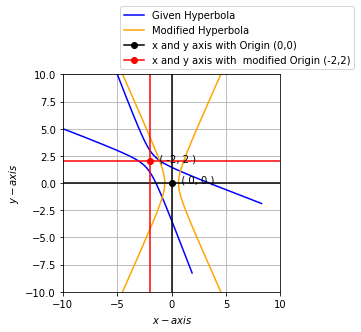
\includegraphics[width=\columnwidth]{hyberbola.png}
	\caption{Hyperbola plot when origin is shifted}
	\label{myfig}
\end{figure}
\end{document}
